\subsection{Analyze parallel algorithms}

Whether we want to analyze our parallel algorithm created with the PCAM model or evaluate a general parallel algorithm, we need some metrics.

\highspace
The classical \textbf{metrics} needed to evaluate a parallel algorithm are:
\begin{itemize}
    \item \textbf{Time complexity}: quantifies the amount of \textbf{time required to produce a solution}.
    \item \textbf{Resource complexity}: quantifies how many \textbf{resources are needed to produce the solution in that time}.
\end{itemize}
In general, to analyze a \textbf{parallel algorithm}, we can consider its \textbf{structure as a directed acyclic graph (DAG)}\footnote{A \definition{Directed Acyclic Graph (DAG)} is a directed graph, i.e. with oriented edges, without cycles.}, where the nodes are the task and the edges are the data dependencies.

\highspace
\begin{flushleft}
    \textcolor{Red2}{\faIcon{book} \textbf{Parallel Algorithm Terminology and Metrics}}
\end{flushleft}
\begin{itemize}
    \item \definitionWithSpecificIndex{Concurrent tasks}{Concurrent tasks in parallel algorithms}{}, each task is executed \emph{\textbf{independently}}.
    
    \item \definitionWithSpecificIndex{Parallel tasks}{Parallel tasks in parallel algorithms}{}, each task is executed at the \emph{\textbf{same time}} (because multiple computing resources are available).
    
    \item \definitionWithSpecificIndex{Work $W$}{Work metric for parallel algorithms}{} is the \emph{\textbf{number of operations executed}}. It may be higher than the sequential version of the algorithm due to communication overhead, etc.
    
    \item \definitionWithSpecificIndex{Span $S$}{Span metric for parallel algorithms}{} is the \emph{\textbf{longest chain of dependencies}} (i.e., the critical path) that determines the \emph{\textbf{minimum time required to execute the algorithm}}. This is a \emph{lower bound} on the running time, regardless of the number of processors. The range indicates the ability of an algorithm to get better performance on more processors.
    \begin{flushleft}
        \textcolor{Green3}{\faIcon{question-circle} \textbf{How do we calculate the Span metric?}}
    \end{flushleft}
    \begin{enumerate}
        \item As we just said, we \textbf{represent a parallel algorithm as a DAG} graph, where nodes represent tasks and edges represent dependencies between tasks;
        \item We \textbf{assign weights to each node} that represent the \textbf{time required to perform the corresponding task};
        \item We try to \textbf{find the Critical Path}. In other words, we determine the path from the start node to the end node that has the \emph{maximum cumulative weight};
        \item Finally, the \textbf{sum} of the \textbf{weights of the nodes on the critical path} gives us the span value!
    \end{enumerate}

    \newpage
    \item \definitionWithSpecificIndex{Parallelism $P$}{Parallelism metrico for parallel algorithms}{} is the \emph{\textbf{measure of efficiency in the use of resources}}. Trivially, it is the number of operations performed divided by the longest chain of dependencies:
    \begin{equation}
        P = \dfrac{W}{S}
    \end{equation}
    It indicates \textbf{how many processors can be effectively used by the computation}. If the work is equal to the span, the parallelism is 1 and the computation is sequential. Ideally, but not necessarily, we win with polylogarithmic span, because if the work is $O(n \log n)$ and the span is $O(\log^{2} n)$, then the parallelism is $O\left(\frac{n}{\log n}\right)$, which is actually quite high (and unlikely to be a bottleneck on most machines in the next 25 years).\cite{introductionToParallelAlgorithmsUMD}

    This measure is \emph{one of the most important}. It indicates the \textbf{number of processors that are not idle}. It is obvious that a \textbf{good parallel algorithm is designed to have the lowest possible work} (less operation, then less resource usage, then less cost, and so on) \textbf{and the highest possible parallelism} (achievable by reducing the span, and this should be trivial, since the metric $P$ is given by work divided by the span, so reducing the denominator, you can get a higher value).

    As in all things, there is a \textbf{trade-off} between the lowest possible \dquotes{work} and the highest possible \dquotes{parallelism}. Reducing the work too much could eliminate the possibility of parallelizing our algorithm, and on the other hand, reducing the span too aggressively could cause communication/synchronization overhead.
\end{itemize}

\begin{figure}[!htp]
    \centering
    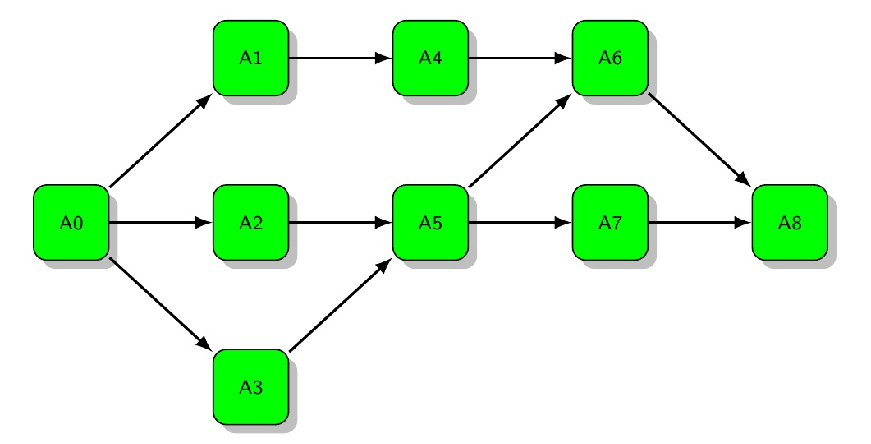
\includegraphics[width=.7\textwidth]{img/dag-1.pdf}
    \caption{Example of DAG implementation with work equal to 9, span equal to 5, and parallelism equal to 1.8 ($9 \div 5$). The span calculus is not well known, has been calculated \emph{a priori}.}
\end{figure}

\noindent
Finally, we use a mathematical annotation and not only a graphical (DAG) annotation. The \definition{Composition Rules} help determine how to combine smaller parallel tasks into a larger algorithm, while analyzing the Work and Span of the combined algorithm:
\begin{itemize}
    \item \textbf{Single operation}. An operation takes 1 unit of work and 1 unit of span time.
    \begin{equation*}
        W\left(op\right) = 1 \hspace{2em} S\left(op\right) = 1
    \end{equation*}

    \newpage

    \item \textbf{Sequential Composition}.
    \begin{itemize}
        \item The total work of executing $e_{1}$ and $e_{2}$ \textbf{sequentially} is the sum of their individual work.
        \begin{equation*}
            W\left(e_{1}, e_{2}\right) = W\left(e_{1}\right) + W\left(e_{2}\right)
        \end{equation*}

        \item The total span of executing $e_{1}$ and $e_{2}$ \textbf{sequentially} is the sum of their individual spans.
        \begin{equation*}
            S\left(e_{1}, e_{2}\right) = S\left(e_{1}\right) + S\left(e_{2}\right)
        \end{equation*}
    \end{itemize}
    
    \item \textbf{Parallel Composition}.
    \begin{itemize}
        \item The total work of executing $e_{1}$ and $e_{2}$ in \textbf{parallel} is still the sum of their individual works.
        \begin{equation*}
            W\left(e_{1} || e_{2}\right) = W\left(e_{1}\right) + W\left(e_{2}\right)
        \end{equation*}

        \item The total span of executing $e_{1}$ and $e_{2}$ in \textbf{parallel} is the \emph{\textbf{maximum of their individual spans}}, since they can be executed simultaneously.
        \begin{equation*}
            S\left(e_{1} || e_{2}\right) = \max\left(W\left(e_{1}\right), W\left(e_{2}\right)\right)
        \end{equation*}
    \end{itemize}
\end{itemize}